\section{问题三:文物类别的鉴别与模型稳健性分析}

本章的核心任务是应用分类模型对未知类别玻璃文物的化学成分进行分析,确定其所属类型,并对分类结果的稳健性与可靠性进行系统性验证。为完成此任务,我们首先进行了一系列对比实验以选择最合适的模型架构,随后采用改进遗传算法对所选模型的超参数进行寻优,构建最终的分类器。最后,我们使用该模型进行预测,并通过双重灵敏度分析来检验结论的稳定性。其整体框架如图\ref{fig:model_framework}所示。

\begin{figure}[H]
    \centering
    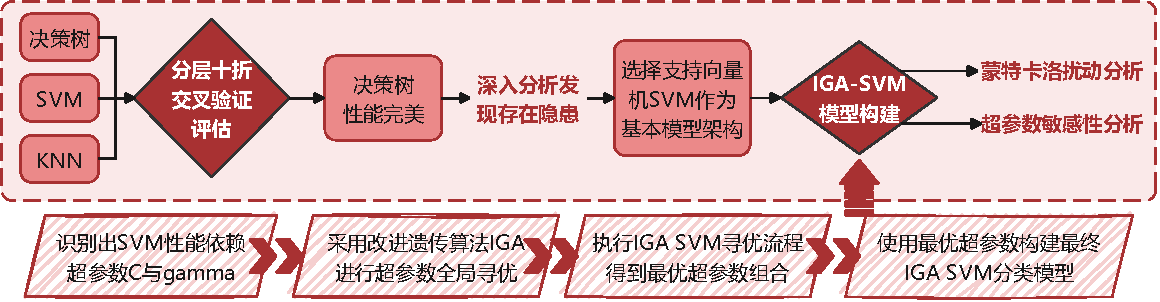
\includegraphics[width=\textwidth]{figs/5问题三/第三问框架.pdf}
    \caption{分类模型框架}
    \label{fig:model_framework}
\end{figure}

\subsection{分类模型的选择与论证}

为建立有效的分类规律,需要从多种候选模型中筛选出最适宜本数据特性的算法。我们选取决策树,K近邻算法以及支持向量机三种具有代表性的模型,在包含全部十四种化学成分及表面风化状况的完整特征集上进行初步性能评估。评估过程采用分层十折交叉验证方法,以保证每次训练与测试中样本类别的分布与原始数据保持一致。各模型的性能指标如表\ref{tab:model_performance}所示。

\begin{table}[H]
    \centering
    \caption{初步模型性能评估}
    \label{tab:model_performance}
    \begin{tabular}{lcc}
        \toprule
        \textbf{模型} & \textbf{准确率} & \textbf{F1分数} \\
        \midrule
        决策树 & 1.0000 & 1.0000 \\
        SVM & 0.9714 & 0.9576 \\
        KNN & 0.9857 & 0.9788 \\
        \bottomrule
    \end{tabular}
\end{table}

评估结果表明,决策树模型在所有性能指标上均达到了1.0的满分。为探究决策树模型取得此结果的原因,我们对其内部结构进行了分析。通过在完整的已分类数据集上训练单个决策树模型,我们发现其特征重要性得分几乎全部集中于氧化铅$PbO$这一项上。模型的可视化结构进一步确认了此发现,如图\ref{fig:decision_tree_structure}所示,该决策树仅在根节点依据氧化铅$PbO$含量是否大于一个特定阈值便完成了对所有样本的分类。

\begin{figure}[H]
    \centering
    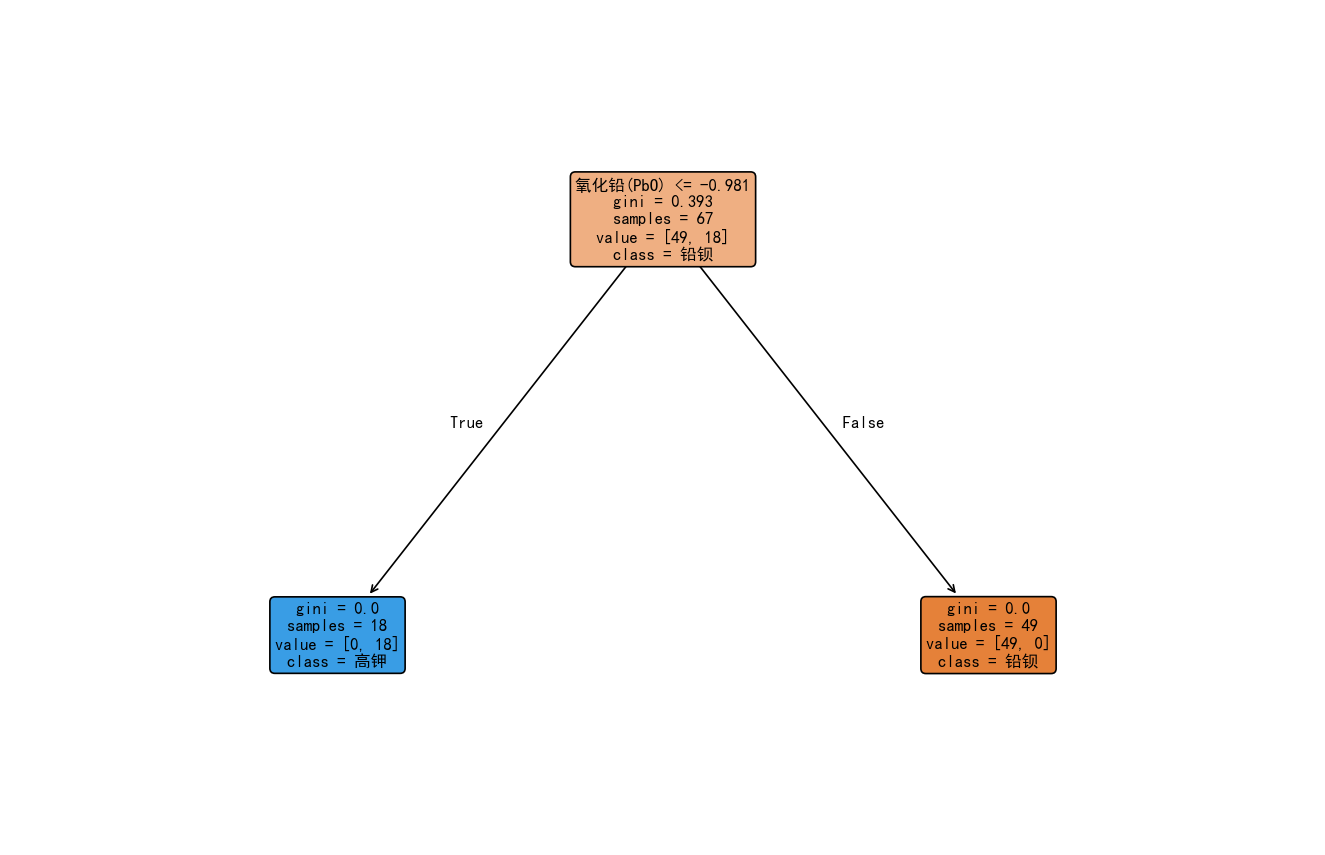
\includegraphics[width=0.8\textwidth]{figs/5问题三/初步决策树可视化图.png}
    \caption{初步决策树模型结构}
    \label{fig:decision_tree_structure}
\end{figure}

尽管决策树表现出很高的评分,但其过分依赖单一特征的决策模式存在稳健性隐患。一个仅凭氧化铅含量进行判断的模型,在面对不含氧化铅但仍属铅钡玻璃体系的未知样本时可能失效,其泛化能力不足。同时,由于该特征的存在,不同模型间的性能差异被掩盖,使得模型对比失去参考价值。基于这些考量,我们排除了将决策树作为最终模型的方案,转而寻求更能利用多维度信息且结构更为稳健的模型。在移除氧化铅特征后进行的补充实验中,支持向量机表现出优越的适应能力,因此我们选择支持向量机作为最终模型的基本架构。

\subsection{基于改进遗传算法的支持向量机模型构建}

支持向量机是一种在高维空间中寻找最优分类超平面的算法,其性能表现高度依赖于正则化系数$C$和核函数系数$\gamma$这两个超参数的设定。为充分发挥支持向量机的性能,我们采用改进遗传算法IGA来代替传统的网格搜索,对其超参数组合进行智能化全局寻优。

支持向量机的基本原理可表述为求解一个软间隔优化问题,其目标函数如下
\begin{equation}
    \min_{\boldsymbol{w}, b, \boldsymbol{\xi}} \frac{1}{2} ||\boldsymbol{w}||^2 + C \sum_{i=1}^{m} \xi_i
\end{equation}
式中$\boldsymbol{w}$与$b$定义了分类超平面,$\xi_i$是允许样本偏离正确边界的松弛变量,而$C$则用以平衡间隔最大化与分类误差。

改进遗传算法IGA是一种模拟生物进化过程的全局优化算法。它将超参数寻优过程转化为一个适者生存的演化过程。算法首先在预设的参数范围内随机生成一个包含多个个体即多组$C$与$\gamma$参数组合的初始种群。随后,算法以分层十折交叉验证的F1分数为适应度函数,对种群中每个个体的优劣进行评估。适应度越高的个体,在后续的遗传操作中被选中作为父代产生后代的概率越大。通过选择,交叉和变异这三种模拟自然繁殖过程的核心算子,算法不断迭代产生适应度更高的新一代种群。此外,精英保留策略确保了每一代的最优个体都能直接进入下一代,保证了寻优过程的收敛性。当达到预设的进化代数或种群适应度不再提升时,算法终止,并输出整个进化过程中适应度最高的个体所对应的超参数组合作为全局最优解。具体机制如\cref{alg:iga_svm}所示。

\begin{algorithm}[H]
    \caption{改进遗传算法IGA优化支持向量机超参数}
    \label{alg:iga_svm}
    \begin{algorithmic}[1]
        \Require
        \Statex 数据集 $D$
        \Statex 种群大小 $N$
        \Statex 最大进化代数 $G_{max}$
        \Statex 交叉概率 $p_c$
        \Statex 变异概率 $p_m$
        \Statex 超参数搜索空间 $S_C, S_{\gamma}$
        
        \Ensure
        \Statex 最优超参数组合 $(C_{best}, \gamma_{best})$

        \Function{IGA-SVM-Optimization}{$D, N, G_{max}, p_c, p_m, S_C, S_{\gamma}$}
            \State 初始化种群 $P_0$:随机生成 $N$ 个个体 $(C_i, \gamma_i)$,其中 $C_i \in S_C, \gamma_i \in S_{\gamma}$
            \State 定义适应度函数 $Fitness(C, \gamma) \leftarrow$ 使用 $(C, \gamma)$ 配置的SVM在数据集$D$上进行分层十折交叉验证的F1分数
            \For{$g = 1$ \textbf{to} $G_{max}$}
                \State 计算当前种群 $P_{g-1}$ 中每个个体的适应度
                \State $P_{new} \leftarrow \emptyset$ \Comment{初始化新一代种群}
                \State 寻找当前种群中的最优个体 $elite \leftarrow \arg\max_{i \in P_{g-1}} Fitness(i)$
                \State $P_{new} \leftarrow P_{new} \cup \{elite\}$ \Comment{精英保留策略}
                
                \For{$k = 1$ \textbf{to} $N-1$}
                    \State \Comment{通过遗传算子生成新个体}
                    \State $parent_1, parent_2 \leftarrow$ \Call{Select}{$P_{g-1}$} \Comment{根据适应度选择父代}
                    \If{$\text{random}(0,1) < p_c$}
                        \State $child \leftarrow$ \Call{Crossover}{$parent_1, parent_2$} \Comment{交叉操作}
                    \Else
                        \State $child \leftarrow parent_1$ \Comment{直接复制}
                    \EndIf
                    
                    \If{$\text{random}(0,1) < p_m$}
                        \State $child \leftarrow$ \Call{Mutate}{$child$} \Comment{变异操作}
                    \EndIf
                    
                    \State $P_{new} \leftarrow P_{new} \cup \{child\}$
                \EndFor
                \State $P_g \leftarrow P_{new}$ \Comment{更新种群}
            \EndFor
            
            \State $(C_{best}, \gamma_{best}) \leftarrow \arg\max_{i \in P_{G_{max}}} Fitness(i)$ \Comment{找出最终的最优个体}
            \State \Return $(C_{best}, \gamma_{best})$
        \EndFunction
    \end{algorithmic}
\end{algorithm}

在具体实现中,我们配置了一个包含15个个体,进化30代的遗传算法。其寻优过程如图\ref{fig:iga_process}所示,该三维瀑布图展示了在迭代过程中,种群的最高适应度,平均适应度与最低适应度的变化情况。图中可见,种群的整体适应度随着进化代数的增加而快速上升并趋于稳定,表明该算法能够高效地在参数空间中搜索到最优解区域。

\begin{figure}[H]
    \centering
    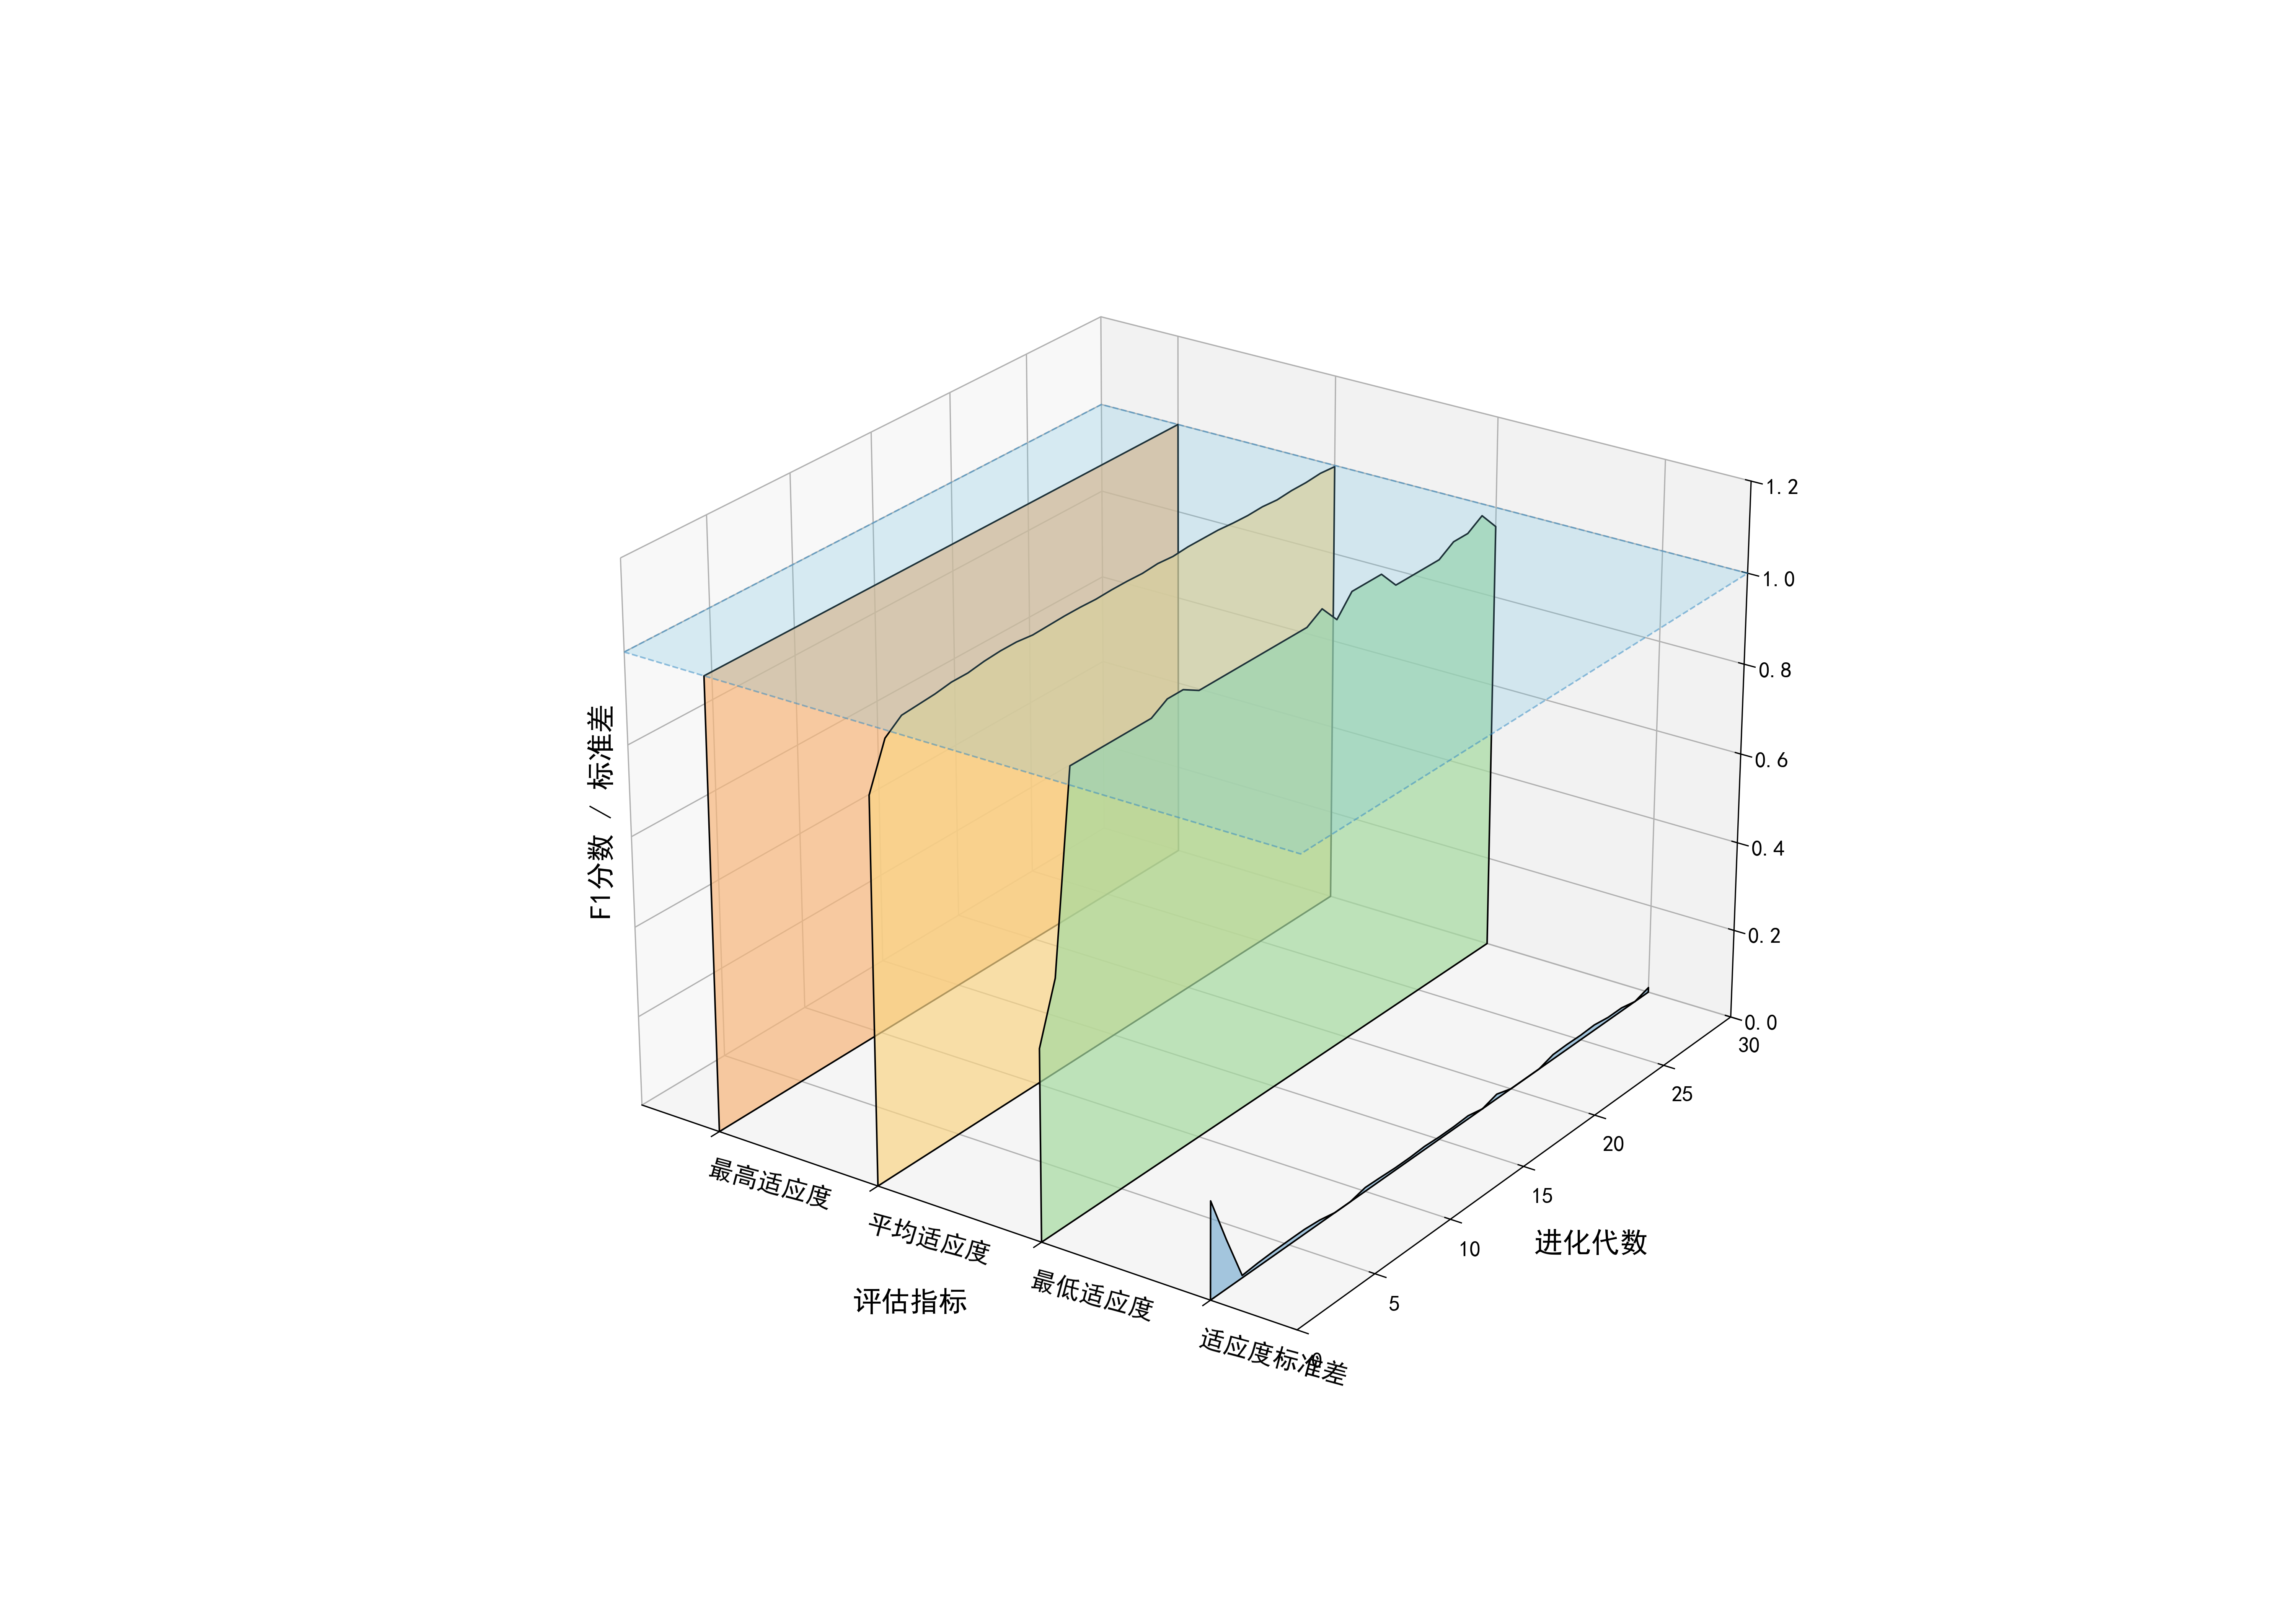
\includegraphics[width=\textwidth]{figs/5问题三/IGA_SVM寻优过程3D瀑布图_最终版.png}
    \caption{改进遗传算法寻优过程}
    \label{fig:iga_process}
\end{figure}

\subsection{最终鉴别结果与双重可靠性验证}

利用前述流程寻得的最优超参数构建最终的IGA-SVM分类模型后,我们将其应用于8个未知类别样本的化学成分数据,完成了最终的类别鉴别。其具体的预测结果如表\ref{tab:prediction_results}所示。

\begin{table}[H]
    \centering
    \caption{未知样本最终预测结果}
    \label{tab:prediction_results}
    \begin{tabular}{|c|c|c|c|c|c|c|c|c|}
        \hline
        \textbf{样本标识} & 0 & 1 & 2 & 3 & 4 & 5 & 6 & 7 \\
        \hline
        \textbf{预测类别} & 高钾 & 铅钡 & 铅钡 & 铅钡 & 铅钡 & 高钾 & 高钾 & 铅钡 \\
        \hline
    \end{tabular}
\end{table}

以确保鉴别结果的可靠性,我们从数据与模型两个维度设计了双重灵敏度分析方案。第一重分析是蒙特卡洛扰动分析,用以检验预测结论对于数据测量误差的稳健性。我们进行了1000次模拟实验,在每次实验中,对样本的部分化学成分数据加入0至5个百分点的随机噪声,然后使用模型重新进行预测。我们通过计算每个样本预测结果在1000次扰动中发生改变的频率,来量化其预测不稳定性。实验结果显示,所有样本的预测不稳定性得分均为0,这表明鉴别结论对于一定范围内的测量误差具有高度的稳定性。

第二重分析是支持向量机超参数敏感性分析,用以检验预测结论对于模型参数选择的稳健性。我们围绕寻得的最优$C$与$\gamma$值构建了一个5乘5的参数网格。对于网格中的每一对参数组合,我们都重新训练支持向量机模型并对未知样本进行预测,然后记录其预测结果与原始最优模型结果不一致的样本数量。分析结果通过热力图进行可视化,如图\ref{fig:svm_sensitivity}所示。

\begin{figure}[H]
    \centering
    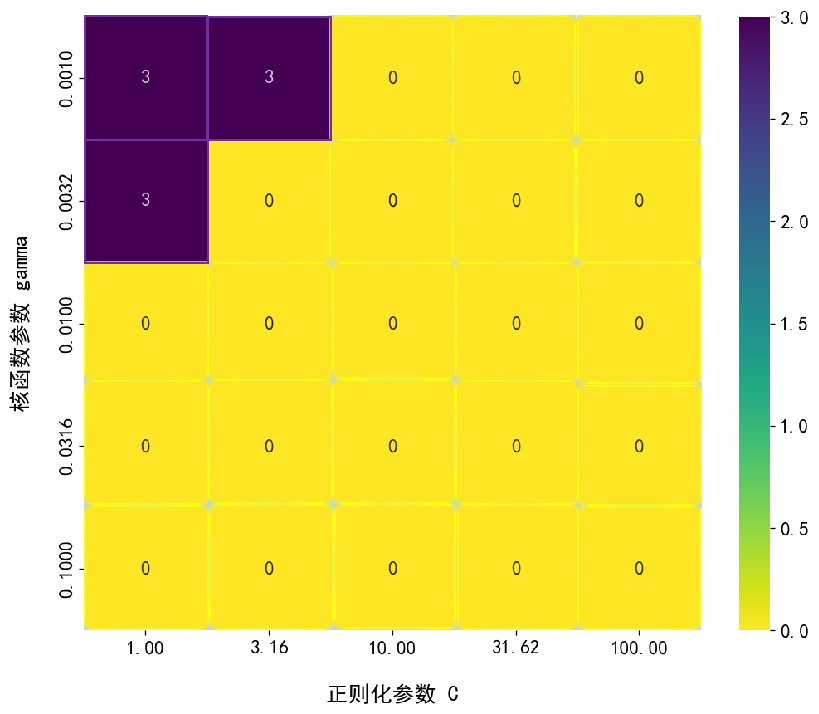
\includegraphics[width=0.7\textwidth]{figs/5问题三/SVM超参数敏感性分析热图.png}
    \caption{支持向量机超参数敏感性分析}
    \label{fig:svm_sensitivity}
\end{figure}

图\ref{fig:svm_sensitivity}中,每个方格的颜色代表在该参数对下预测结果发生改变的样本数量,颜色越深表示变化越大。图中可见,在以最优参数点为中心的广大区域内,颜色均为最浅色,对应数值为0,这意味着预测结果没有发生任何改变。这一广阔的稳定区域证明,最终的鉴别结论对模型超参数的选择不敏感,并非是在某个特定参数点上偶然获得的结果,从而进一步确认了结论的可靠性。
